% !TEX program = XeLaTeX
\documentclass{VUMIFPSkursinis}
    \usepackage{algorithmicx}
    \usepackage{algorithm}
    \usepackage{algpseudocode}
    \usepackage{amsfonts}
    \usepackage{amsmath}
    \usepackage{bm}
    \usepackage{caption}
    \usepackage{color}
    \usepackage{enumitem}
    \usepackage{float}
    \usepackage{graphicx}
    \usepackage{listings}
    \usepackage{subfig}
    \usepackage{wrapfig}
    % Titulinio aprašas
    \university{Vilniaus universitetas}
    \faculty{Matematikos ir informatikos fakultetas}
    \department{Programų sistemų katedra}
    \papertype{Laboratorinis darbas}
    \title{Skrydžių bilietų paieškos sistema}
    \titleineng{Plane tickets search system}
    \status{2 kurso 4 grupės studentai}
    \author{Vardenis Pavardenis}
    \secondauthor{Vardenis Pavardenis}
    \thirdauthor{Vardenis Pavardenis}
    \fourthauthor{Vardenis Pavardenis}
    \date{Vilnius – \the\year}
    
    % Nustatymai
    % \setmainfont{Palemonas}   % Pakeisti teksto šriftą į Palemonas (turi būti įdiegtas sistemoje)
    \bibliography{bibliografija}
    
    \begin{document}
    \maketitle
      
        \tableofcontents
      
        \sectionnonum{Įvadas}
      
        \section{Reikalavimai}
            \subsection{Funkciniai reikalavimai}
                \begin{enumerate}[label=\textbf{FR\arabic*}.]
                    \item Funkcinis...
                \end{enumerate}
            \subsection{Nefunkciniai reikalavimai}
                \begin{enumerate}[label=\textbf{NFR\arabic*}.]
                    \item Turi būti palaikoma operacinė sistema su viena iš naršyklių:
                    \begin{itemize}
                        \item Mozilla Firefox (nuo 58 versijos)
                        \item Google Chrome (nuo 64 versijos)
                        \item Microsoft Internet Explorer (nuo 11 versijos)
                        \item Microsoft Edge (nuo 41 versijos)
                        \item Apple Safari (nuo 11 versijos)
                    \end{itemize}
                    \item Turi būti palaikomas HTTPS standartas.
                    \item Programų sistema turi būti susieta su avia kompanijų bilietų pirkimo svetaine.
                    \item Programų sistema turi turėti prieigą prie duomenų bazes, kurioje saugomi tvarkaraščiai, naudotojai, įvykiai ir užrašai.
                    \item Programų sistema turi būti sukurta naudojant \textit{Angular 5}.
                \end{enumerate}
      
        \section{Struktūrinis dalykinės srities modelis}
            \subsection{Esybių diagrama}
    
            \subsection{Žodynas}
                \begin{enumerate}[label=\textbf{E\arabic*}.]
                    \item Vartotojas - asmuo, norintis nusipirkti skrydžio bilietą.
                    \item Skrydžių bendrovė  - įmonė, kuri suteikia skrydžio paslaugą.
                \end{enumerate}
    
                \begin{table}[H]\footnotesize
                \centering
                \caption{Dalykinės srities metaforų reikalavimai}
                    {\begin{tabular}{|l|l|} \hline
                        Objektas & Metafora \\
                        \hline
                        \hline
                        Paieška & Skrydžių bilietų radimas pagal įvestus paieškos kriterijus \\
                        \hline
                        Rūšiavimas & Maršruto pasirinkimas pagal norimą kriterijų: greitis, kaina, greičio ir kainos santykis \\
                        \hline
                        Filtravimas & Rezultatų pateikimas pagal norimus kriterijus: persėdimų skaičius, skrydžių bendrovės \\
                        \hline
                        Kainų žirklės & Kainos amplitudė \\
                        \hline
                        Užsakymų istorija & Įsigytų skrydžių bilietų peržiūra \\
                        \hline
                        Skrydžių informacija & Įsigytos kelionės duomenys: data, laikas, oro uostai \\
                        \hline
                        Paieškos rezultatai & Gautos užklausos rezultatai \\
                        \hline
                    \end{tabular}}
                \label{tab:table example}
                \end{table}
    
            \subsection{Reikalavimų - struktūrinio dalykinės srities modelio atsekamumo matrica}
            \subsection{Klasių diagrama}
                \begin{figure}[H]
                    \centering
                    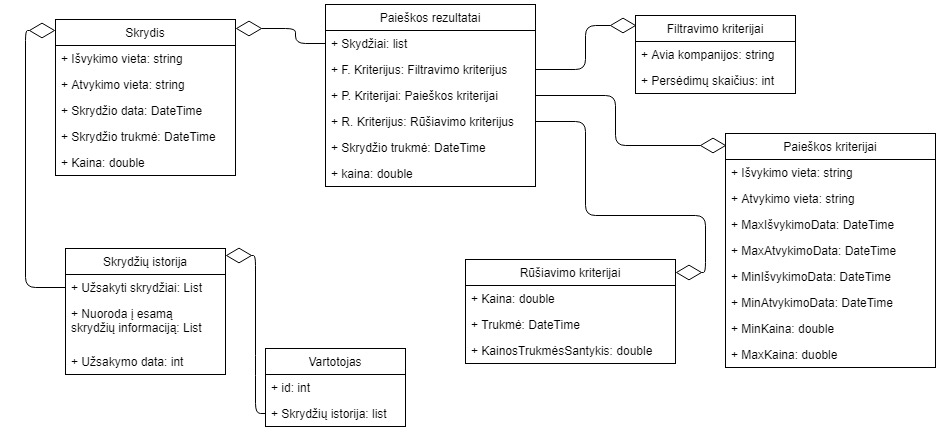
\includegraphics[scale=1]{img/class_diagram}
                    \caption{Klasių diagrama}
                    \label{klasių diagrama}
                \end{figure}
                \begin{enumerate}[label=\textbf{E\arabic*}.]
                    \item Paieškos rezultatai - aprašo skrydžių paieškos rezultatus pritaikius paieškos kriterijus.
                    \item Skrydis - detaliai aprašo skrydžio informaciją. Skrydžio informacija susideda iš išvykimo vietos, atvykimo vietos, skrydžio datos, skrydžio trukmės ir kainos.
                    \item Skrydžių istorija - aprašo vartotojo užsakytų, įvykusių bei būsimų skrydžių informaciją.
                    \item Filtravimo kriterijai - aprašo vartotojo nustatytus filtravimo kriterijus. Vartotjas gali pasirinkti norimas avia kompanijas ir pageidaujamų persėdimų skaičių
                    \item Paieškos kriterijai - aprašo vartotojo pasirinktus skrydžio bilietų paieškos kriterijus. Vartotojas gali nustatyti išvykimo vietą, atvikimo vietą, maksimalią ir minimalią išvykimo bei atvykimo datą, maksimalią bei minimalią kainą.
                    \item Vartotojas - asmuo naviguojantis skrydžių paieškos platformoje ir ieškantis reikiamų skrydžių.
                \end{enumerate}
      
        \section{Užduotys}
            \subsection{Užduočių aprašymai}
            
                \begin{enumerate}[label=\textbf{U\arabic*}.]

                    \item \textbf{Ieškoti skrydžių}\\
                    Vartotojas įveda išvykimo, atvykimo miestus. Pagal pageidavimą, įveda išvykimo ir atvykimo tinkamų laikų intervalus, kainos intervalą. Tada vartotojas paspaudžia ant mygtuko "Ieškoti" ir yra nukreipiamas į paieškos rezultatų langą, kur jam, lentelės pavidalu rodomi surasti skrydžiai pagal vartojojo įvestus kriterijus.
                    \\\textbf{Alternatyvūs scenarijai:}
                    \begin{itemize}
                        \item Jei vartotojas neįveida atvykimo ir/ar išvykimo miestų, jam paspaudus ant mygtuko "Ieškoti" jis nėra nukreipiamas į rezultatų langą. Išvykimo ar atvykimo miesto įvedimo laukas su neįvesta reikšme (arba abu), paženklinami raudonai.
                    \end{itemize}

                    \item \textbf{Rušiuoti paieškos rezultatus}\\
                    Paieškos rezultatų lange, vartotojas pasirenka vieną iš trijų rušiavimo būdus atitinkančių mygtukų: "Greičiausias", "Pigiausias" arba "Optimalus". Paspaudus ant vieno iš jų, skrydžių paieškos rezultatai yra surūšiuojami pagal pasirinktą rušiavimo būdą.
                    \\\textbf{Alternatyvūs scenarijai:}
                    \begin{itemize}
                        \item Surušiavus rezultatus tam tikru pasirinktu būdu, vartotojas paspaudžia ant jau pasirinktą rušiavimo būdą atitinkančio mygtuko. Rezultatai lieka suruošiuoti taip pat kaip ir prieš spaudžiant. 
                    \end{itemize}

                    \item \textbf{Filtruoti paieškos rezultatus}\\
                    Paieškos rezultatų lange, vartotojas pažymi jį dominantį persėdimų skaičių ir skrydžių bendrovę. Vartotojui pažymėjus konkrečią reikšmę ar to, ar ano, paieškos rezultatai yra iš karto atnaujinami, vaizduojant tik tuos skrydžius, kurie tenkina filtrų reikšmes.
                    \\\textbf{Alternatyvūs scenarijai:}
                    \begin{itemize}
                        \item Vartotojui pakartotinai paspaudus ant jau prieš tai pažymėta filtro reikšmės, rezultatai iš karto atsinaujina, o konkretus pažymėtas filtras nuimamas. Kai visi filtrai yra nuimti, rezultatai atsivaizduoja netaikant jiems jokio filtravimo.
                    \end{itemize}

                    \item \textbf{Peržiūrėti detalią skrydžio informaciją}\\
                    Scenarijus
                    \\\textbf{Alternatyvūs scenarijai:}
                    \begin{itemize}
                        \item Scenarijus
                    \end{itemize}

                    \item \textbf{Pereiti į bilieto pardavėjo svetainę}\\
                    Scenarijus
                    \\\textbf{Alternatyvūs scenarijai:}
                    \begin{itemize}
                        \item Scenarijus
                    \end{itemize}

                    \item \textbf{Peržiūrėti būsimų skrydžių sąrašą}\\
                    Scenarijus
                    \\\textbf{Alternatyvūs scenarijai:}
                    \begin{itemize}
                        \item Scenarijus
                    \end{itemize}
                    
                \end{enumerate}
      
            \subsection{Reikalavimų - užduočių atsekamumo matrica}
      
        \sectionnonum{Išvados}
      
        \sectionnonum{Šaltiniai}
    
        \appendix  % Priedai
        % Prieduose gali būti pateikiama pagalbinė, ypač darbo autoriaus savarankiškai
        % parengta, medžiaga. Savarankiški priedai gali būti pateikiami ir
        % Priedai taip pat numeruojami ir vadinami. Darbo tekstas
        % su priedais susiejamas nuorodomis.
      
    \end{document}
      